\section{Introduction}

Recently Linux container clusters draw much attention because they are lightweight, portable and repeatable.
Container clusters are generally more lightweight than Virtual Machine clusters, 
because the containers share the kernel with host OS, still having separate execution environment . 
They are generally portable because the process execution environments are packed
into the tar archives.
Whenever one attempts to run a container, the exact same file systems are restored from the archives, 
even on totally different data centers. 
This means a container cluster can provide the repeatable execution environment.

For WEB services, the Linux containers are attractive because of the same reasons. 
Furthermore, it is expected that WEB systems consisting of container cluster are 
capable of being easily migrated for Disaster Recovery purposes or for other business requirements.


The Kubernetes\cite{K8s2017} container cluster system is one of the prominent candidates
which enable easy migration of the container clusters.
However the migrations are only easy on limited cloud providers including GCP and AWS, because
the Kubernetes is heavily dependent on external load balancers which is set up by cloud providers on the fly through its API.  

The external load balancer set up by the cloud providers will distribute the incoming traffic to every node server.
The traffic is forwarded again using iptables DNAT\cite{MartinA.Brown2017,Marmol2015} as load balancer with the round-robin manner. 

This does not necessarily work for all cloud provider nor for on-premise data centers.
Because most of them do not have load balancers which is supported by the Kubernetes.
On such environments a static routing for inbound traffic are set up manually with ad hoc manner.

This is far from automation or convenient.
Accordingly, migrating container clusters among those environments will always be a burden.

In order to eliminate the dependency on external load balancer, 
we propose a containerized software load balancer which is deploy-able as a part of container clusters.
We will containerize ipvs\cite{Zhang2000} layer 4 load balancer using existing ingress framework of the Kubernetes cluster. 
We also investigate the feasibility of such load balancer by comparing the performance 
with iptables DNAT load balancer functionality and Nginx load balancer.

Also discussed will be appropriate overlay network settings which enable such load balancers to work properly, 
and techniques to derive the most performance out of such load balancers.

The rest of the paper is organized as follows.
The section \ref{Related Work} highlights related work specifically those deal with container cluster migration, 
software load balancer containerization or a load balancer related tools in the context of container. 
The section \ref{Load balancers in Kubernetes cluster} will explain the problem of the existing architecture and propose our solution.
In the section \ref{Performance Measurement}, experimental conditions and the important parameters 
we considered in the experiment will be described in detail.
Then we will show the result of experiment and discuss the obtained performance characteristics in the section~\ref{Result and Discussion} 
which is followed by the conclusion in the section~\ref{Conclusions}.
  

\section{Related Work}\label{Related Work}
This section highlights related work especially those deal with container cluster migration, 
software load balancer containerization or a load balancer related tools in the context of container. 

Developers of the Kubernetes are trying to add federation\cite{K8sFederation2017} capability 
where multiple Kubernetes clusters are deployed on multiple cloud providers or on-premise data centers 
and are managed via federation apiserver server. However, how each of Kubernetes clusters is run on different type of cloud providers
or in on-premise data centers, especially when the load balancers of such environments are not supported by the Kubernetes, 
seems out of the scope of the project. 
   
As far as the containerization of a load balancers are concerned, there are following related works:
Nginx-ingress\cite{Pleshakov2016,NginxInc2016} utilizes the ingress\cite{K8sIngress2017} capability of the Kubernetes, 
and implements containerized Nginx proxy as a load balancer. The Nginx itself is famous as a high performance web server program,
which also has the functionality of layer 7 load balancer. The Nginx is capable of handling TLS encryption and also capable of  
URI based switching. However the flip side of these is that it is much slower than layer 4 switching.
The upper bound of the performance of the Nginx as a load balancer will not be much better than 
that as a single web server serving lightweight web pages. 
Therefore it is meaningless to use the Nginx as a load balancer in such cases.
 
The kube-keepalived-vip\cite{Prashanth2016} project is trying to use the Linux kernel's load balancer capability, 
called ipvs\cite{Zhang2000} by containerizing the keepalived\cite{ACassen2016} and ipvs. 
The keepalived container is using the daemonsets\cite{K8sDaemonsets2017} framework of the Kubernetes. 
In this case the container is run on every node.
This work is very similar to our proposal in the sense that it uses keepalived and ipvs in container. 
However it does not provide per container cluster load balancer which is portable among different cloud providers.   
Our proposal is to provide a load balancer that is configurable and deploy-able at user's will,
 as a part of container cluster itself not as a port of the Kubernetes cluster infrastructure.  

The swarm mode of the docker\cite{DockerCoreEngineering2016,DockerInc2017} also uses ipvs for internal load balancing,
however it is also considered as built-in load balancer functionality of the docker, 
and is different from our proposal.

There are several other projects where an effort to utilize ipvs in the context of container environment.
The gorb\cite{Sibiryov2015} and the clusterf\cite{Aaltodoc:http://urn.fi/URN:NBN:fi:aalto-201611025433} are daemons 
which setups ipvs in the kernel inside docker container. They utilize information about running container stored in key-value storages
like the etcd\cite{CoreOSEtcd} and the consul\cite{HashiCorpConsul}. 
These has the similar functionality to a combination of keepalived and the Kubernetes ingress controller in our proposal.
These may be usable in our environment in future, but that is beyond the scope of this paper.

The contribution of this paper are followings: 
1) We propose a portable software load balancer 
which is runnable on any cloud provider or on on-premise data centers, 
as a part of container cluster.
2) We discuss feasibility of such a load balancer by comparing the performance.
3) We also discuss about usable overlay network and clarify importance of a technique 
to draw the best performance from such load balancers.  


\section{Load balancers in Kubernetes cluster}\label{Load balancers in Kubernetes cluster}

\subsection{Conventional Architecture}

\begin{figure}
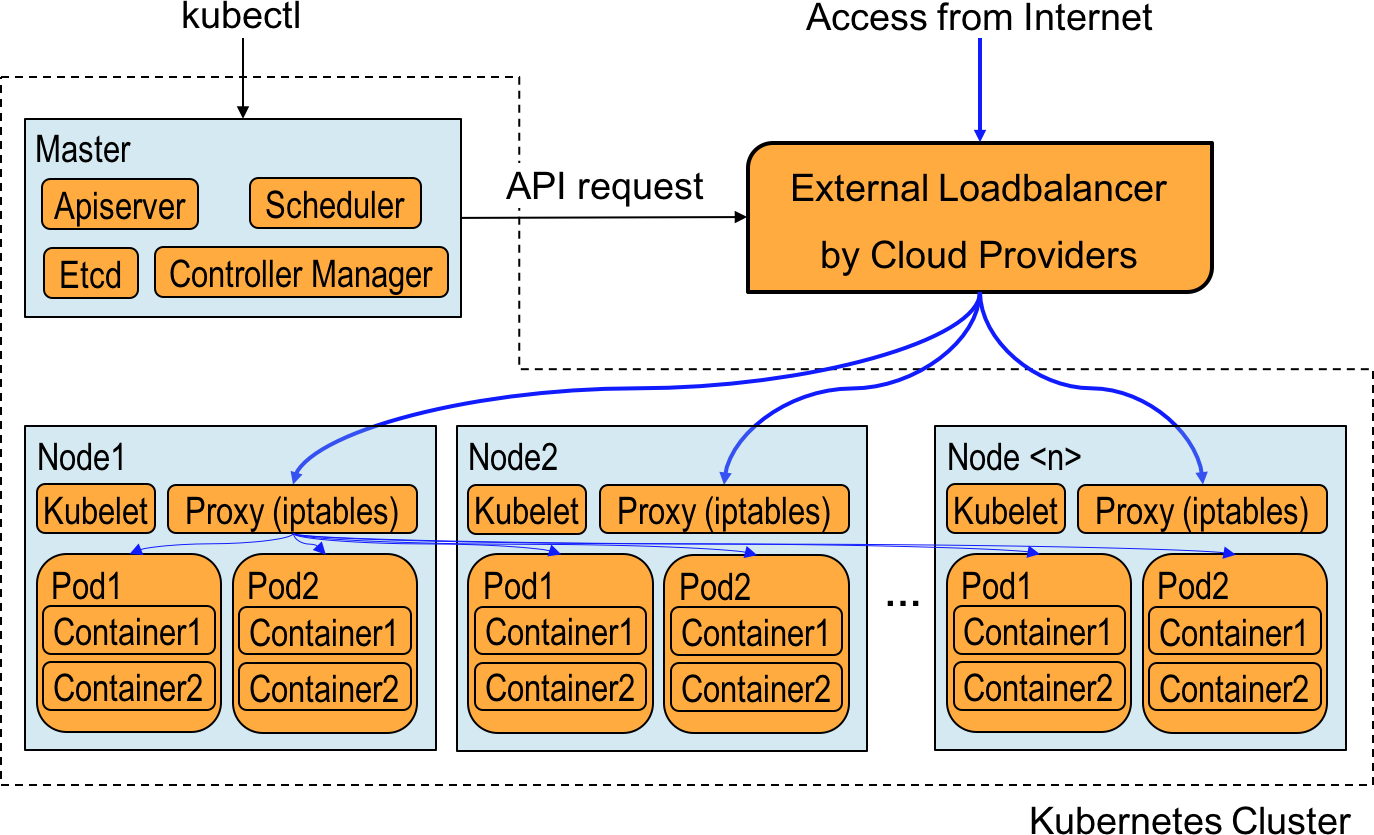
\includegraphics[width=\columnwidth]{Figs/K8sConventional}
\caption{Conventional Architecture of A Kubernetes cluster.}
\label{fig:K8sConventional}
\end{figure}

The Kubernetes container management system has an issue when it is used in outside of recommended cloud providers e.g. GCP or AWS.
Figure~\ref{fig:K8sConventional} shows an exemplified Kubernetes cluster.
The Kubernetes cluster typically consists of master servers and node servers.
On the master servers daemons that control the Kubernetes cluster are typically deployed. 
These daemons include, apiserver, scheduler, controller-manager and etcd. 
On the node servers, the kubelet daemon will run pods, depending the PodSpec information obtained from the apiserver on the master servers.
A pod is a group of containers which share the net name space and cgroups, 
and is the basic execution unit in the Kubernetes cluster.

When a service is created, the masters will send out request to cloud providers API endpoints, 
to set up external load balancers.
The proxy daemon on the node servers will also setup iptables DNAT\cite{MartinA.Brown2017} rules, 
which distributes the inbound traffic to the existing pods.

The traffic from the internet will be distributed by the external load balancer to node servers evenly, 
then it will be distributed again by the DNAT rules on the node serves to designated pods. 
The returning packets will follow the exact same route as the incoming ones.

The problems of this architecture are the followings: 
1) Having external load balancers whose APIs are supported by the Kubernetes daemons is the prerequisite. 
There are many cloud providers where the API of load balancers is not supported by Kubernetes. 
There are many load balancers which dose not even have APIs that is usable by Kubernetes, 
especially for on-premise data centers.  
In such cases, one could manually setup the routing table on a gateway to one of the node servers, 
then the traffic will be distributed by the DNAT rules on the node to designated pods.
However this is far from convenient.
2) Distributing the traffic twice, firstly on the external load balancers and secondary on each node, 
will complicate the route which a packet follows. 
Imagine the situation, where the DNAT table on one of the node servers malfunctions.
In such case, you will only observe occasional timeouts. It is very difficult to find out which node server malfunctions.   

\subsection{Proposed Architecture}

\begin{figure}
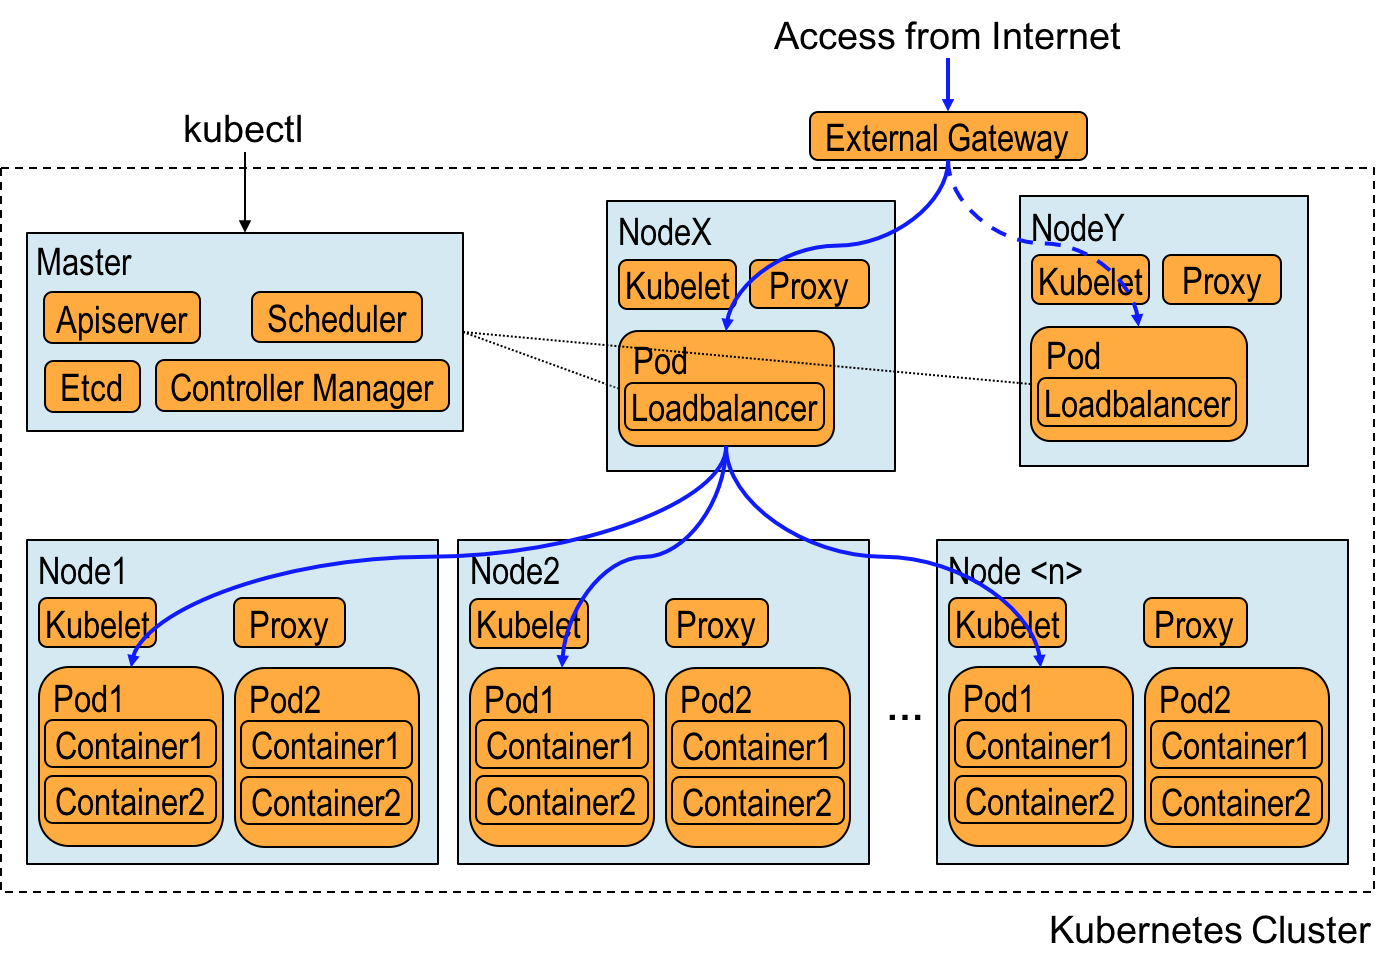
\includegraphics[width=\columnwidth]{Figs/K8sProposed}
\caption{A Kubernetes cluster with proposed load balancer.}
\label{fig:K8sProposed}
\end{figure}

Figure~\ref{fig:K8sProposed} shows the proposed architecture of the Kubernetes cluster, 
which has following characteristics:
1) Each load balancer itself is run as a pod by the Kubernetes. 
2) There exist multiple load balancers for redundancy. 
3) Configuration of the load balancers are dynamically updated depending on the information of running pods.

By following these architecture, we can resolve the problems of conventional architecture.
Since load balancer itself is containerized, it can be run on any environment including on-premise data centers.
And because it only distribute traffic only once on the load balancer, it is relatively easy to find malfunctions.

In this paper, we propose a containerized software load balancer. 
Specifically we will implement a container which setup Linux kernel's load balancer functionality, 
ipvs inside the container's net name space.
We also discuss the feasibility of the proposed load balancer by comparing the performance with existing iptables and Nginx based load balancer. 


\subsection{Implementation}\label{Implementation}

\begin{figure}
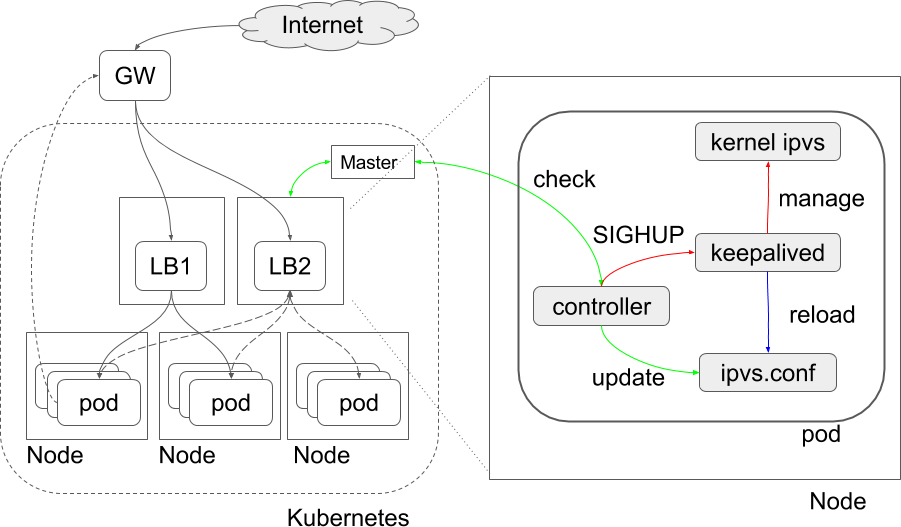
\includegraphics[width=\columnwidth]{Figs/ipvs-ingress-schem}
\caption{Implementation}
\label{fig:ipvs-ingress-schem}
\end{figure}

Figure~\ref{fig:ipvs-ingress-schem} show the schematic diagram of a container that functions as a load balancer.
Inside the container, two daemons, controller and keepalived are run.
The keepalived is a program which modifies Linux kernels ipvs rules depending on the configuration file, ipvs.conf.
The keepalived is also capable of health-checking the liveliness of real-server, 
which is a combination of IP address and port number of the target pods. 
If the health-check to a real server fails, the keepalived will remove that real server from the ipvs rules.

The controller monitors information of running pods of a service in the Kubernetes cluster by consulting the apiserver on the master server.
Whenever pods are created or deleted, it will automatically regenerate appropriate ipvs.conf and issue SIGHUP to the keepalived.
Then the keepalived will reload the ipvs.conf and modify the kernel's ipvs rules.  

The actual controller\cite{ktaka_ccmp_2017_826894} has been implemented using ingress controller\cite{K8sIngress2017} framework of the Kubernetes.
By importing existing Golang package, \enquote{k8s.io/ingress/core/pkg/ingress},
we only needed 120 lines of code.  

In this way, the ipvs's balancing rules inside Linux kernel are maintained so that it could distribute the incoming traffic only to the living pods.

In order to let the kernel to load required kernel modules inside a container, 
we needed to add the CAP\_SYS\_MODULE capability to the container, 
and also needed to mount the \enquote{/lib/module} of the node's file system on the container's file system.   
In order to let the keepalived manipulate kernel's ipvs rules, 
we needed to add CAP\_NET\_ADMIN capability to the container.

There is an explanation in \cite{mp2016enhancing} about some of the capabilities 
that is usually dropped inside docker containers.

\begin{figure}
\begin{minipage}{0.7\columnwidth}
\begin{verbatim}

virtual_server fwmark 1 {
  delay_loop 5
  lb_algo lc
  lb_kind NAT
  protocol TCP
  real_server 172.16.21.2 80 {
    uthreshold 20000
    TCP_CHECK {
      connect_timeout 5
      connect_port 80
    }
  }
  real_server 172.16.80.2 80 {
    uthreshold 20000
    TCP_CHECK {
      connect_timeout 5
      connect_port 80
    }
  }
}

\end{verbatim}
\end{minipage}
\caption{An example of ipvs.conf}
\label{fig:ipvs.conf}
\end{figure}

\begin{figure}
\begin{minipage}{\columnwidth}
\small
\begin{verbatim}

# kubectl exec -it ipvs-controller-4117154712-kv633 -- ipvsadm -L
IP Virtual Server version 1.2.1 (size=4096)
Prot LocalAddress:Port Scheduler Flags
  -> RemoteAddress:Port Forward Weight ActiveConn InActConn
FWM  1 lc
  -> 172.16.21.2:80      Masq    1      0          0         
  -> 172.16.80.2:80      Masq    1      0          0

\end{verbatim}
\end{minipage}
\caption{An example of ipvs balancing rules}
\label{fig:ipvs rule}
\end{figure}

Figure~\ref{fig:ipvs.conf} shows an example of ipvs.conf file generated by the controller. 
Shown in Figure~\ref{fig:ipvs rule} is the corresponding ipvs's load balancing rules.
We can see that the packet with {\tt fwmark=1}\cite{BertHubert2002} is distributed 
to the {\tt 172.16.21.2:80} and {\tt 172.16.80.2:80} 
using the masquerade mode(Masq)\cite{Zhang2000} and 
the least connection(lc)\cite{Zhang2000} balancing algorithm.   

\section{Performance Measurement}\label{Performance Measurement}

We carried out performance measurement of the proposed load balancer using benchmark program called, wrk\cite{Glozer2016}.
We also measured performance of iptables's DNAT load balancing functionality and Nginx layer 7 load balancer for comparison.

When creating Kubernetes cluster, an overlay network\cite{Sill2016,Marmol2015} is often used. 
Among available overlay networks, the flannel\cite{CoreOSFlannel} is a popular one.
We compared each of the three backends\cite{CoreOSFlannelBackend}, 
{\it i.e.} operating modes of the flannel by the benchmark of the load balancers.

It is known that distributing the handling of interrupts from the NIC 
and the following IP protocol processing, among multiple cores are important.

In order to derive the best performance from a load balancer, 
we also investigated how this would affect the performance of load balancers.

\subsection{Benchmark method}

\begin{figure}
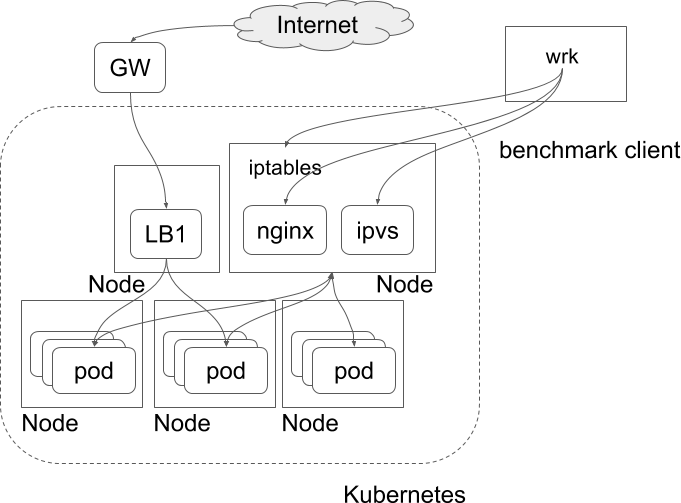
\includegraphics[width=\columnwidth]{Figs/benchmark-schem}
\caption{Benchmark setup}
\label{fig:benchmark-schem}
\end{figure}

Using the wrk, we measured performance of the load balancers.
Figure~\ref{fig:benchmark-schem} shows schematic diagram of the experimental setups.
Having deployed pods running Nginx web servers which returns IP address of the pod itself,
we set up the ipvs, iptables and Nginx load balancers on one of the node servers. 

The HTTP GET requests are sent out by the wrk on the client machine toward the node servers.
The destination IP address and port number is chosen 
depending on the type of the load balancer on which the measurement is performed.
The load balancer on the node server then distribute the requests to the pods.
Each pod will return HTTP responses to the load balancer and the load balancer will then return the response to the client.

The number of responses received by the wrk on the client is counted, 
then the performance in terms of the request/sec is obtained. 

Figure~\ref{fig:benchmark example} shows an example of the command-line for the wrk and the corresponding output.
The command-line in Figure~\ref{fig:benchmark example} will generate 40 threads of wrk program 
and lets those threads send out in total of 800 concurrent HTTP requests during 30 seconds.

The example output shows information including per thread statistics, error counts, Request/sec and Transfer/sec[MByte/sec].
We considered the \enquote{Request/sec} to be the performance, and compared for several conditions.

Figure~\ref{fig:Hardware and software configuration} shows hardware and software configuration used in our experiments.
We used Nginx as the target HTTP server which returns own IP address as HTTP content. 
The size of the characters of an IP address is only up to 15 bytes, 
which is relatively severe condition for a load balancer.
If we chose the size of the HTTP response so that most of the IP packet result in MTU,
the benchmark results would be limited by the bandwidth of the Ethernet.
Since we used smaller HTTP responses, we could perform the severer benchmark against load balancers than otherwise.

\begin{figure}
\begin{minipage}{\columnwidth}
\small
\begin{Verbatim}[commandchars=\\\{\}]

\underline{\textbf{Command line:}}
 wrk -c800 -t40 -d30s http://172.16.72.2:8888/
-c: concurrency, -t: # of thread, -d: duration

\underline{\textbf{Result sample:}}
 Running 30s test @ http://10.254.0.10:81/
  40 threads and 800 connections
  Thread Stats   Avg      Stdev     Max   +/- Stdev
    Latency    15.82ms   41.45ms   1.90s    91.90%
    Req/Sec     4.14k   342.26     6.45k    69.24%
  4958000 requests in 30.10s, 1.14GB read
  Socket errors: connect 0, read 0, write 0, timeout 1
Requests/sec: 164717.63
Transfer/sec:     38.86MB

\end{Verbatim}
\end{minipage}
\caption{An example output of benchmark by wrk}
\label{fig:benchmark example}
\end{figure}

\begin{figure}
\begin{minipage}{0.9\columnwidth}
\small
\begin{Verbatim}[commandchars=\\\{\}]

\underline{\textbf{Physical Machine Specification:}}
  CPU: Intel(R) Xeon(R) CPU E5-2450 0 @ 2.10GHz
  # of Physical Cores: 8
  Hyper Threading: enabled
  Memory: 32GB
  NIC: Broadcom BCM5720 Gigabit Ethernet PCIe

\underline{\textbf{Number of Physical Machines:}}
  Master: 1
  Node: 7
  Client: 1

\underline{\textbf{Node Software version:}}
  OS: Debian 8.7 (Jessie)
  Kernel: \footnotesize{3.16.0-4-amd64 #1 SMP Debian 3.16.39-1 (2016-12-30)}
  Kubernetes v1.5.2
  flannel v0.7.0
  etcd version: 3.0.15

\underline{\textbf{Load balancer Software version:}}
  Keepalived: v1.3.2 (12/03,2016)
  Nginx: nginx/1.11.1

\underline{\textbf{Worker Pod Software version:}}
  nginx : nginx/1.13.0 

\end{Verbatim}
\end{minipage}
\caption{Hardware and software configuration}
\label{fig:Hardware and software configuration}
\end{figure}


\subsection{Overlay network}

When building a Kubernetes cluster, one has a choice in usable overlay networks.
We used the flannel to build the Kubernetes cluster used in our experiment. 
The flannel has 3 types of backend {\it i.e.} operating mode, called host-gw, vxlan and udp\cite{CoreOSFlannelBackend}.

In the host-gw mode, the flanneld on a node server simply set up the routing table 
based on IP address assignment information of the overlay network which is stored in etcd. 
When a pod on a node sends out a IP packet to another pods on a different node server, 
the former node servers will consult the routing table and learn that that IP packet should be sent out to the latter node.
Then the former node will form Ethernet frames having destination MAC address of the latter node without changing the IP header.

In the case of the vxlan mode, the flanneld will create Linux kernel's vxlan device, flannel.1. 
The flanneld also setup the routing table appropriately based on the information stored in the etcd.
When pods on different nodes need to communicate, the packet is routed to flannel.1.
The vxlan functionality of the Linux kernel will find out MAC address of flannel.1 device on the opponent node server 
then form a Ethernet frame toward that MAC address.
The vxlan will then encapsulate the Ethernet frame in a UDP/IP packet with vxlan header.
The IP packet is sent out eventually.

In the case of udp mode, the flanneld will create a tun device, flannel0 and setup the routing table.
The flannel0 device is connected to flanneld daemon itself.
An IP packet routed to flannel0 is encapsulated bye the flanneld, and eventually sent out 
to the appropriate node server. 
The encapsulation is done for IP packets.

Figure~\ref{fig:flannel-packet-diagram} shows schematic diagrams of frame format for the three backend of 
the flannel overlay network.
Also shown are the MTU sizes of each operation mode, assuming the MTU without encapsulation is 1500byte.

Since packets are not encapsulated in the host-gw mode, the MTU remains 1500bytes.
Additional 50bytes of header is used in vxlan mode, resulting in MTU of 1450bytes.
In the case of udp mode only 28bytes of header is used for encapsulation, which results in MTU of 1472bytes.


\begin{figure}
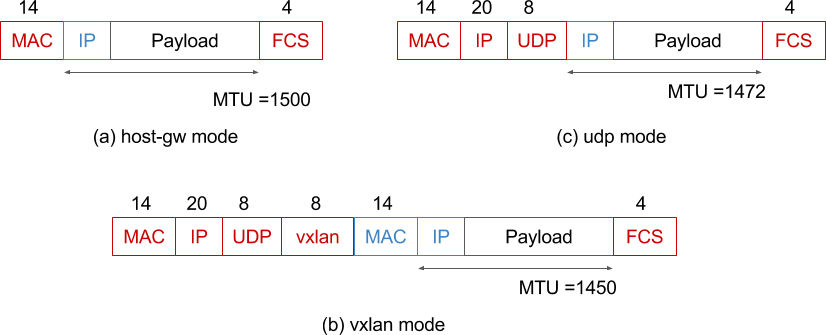
\includegraphics[width=\columnwidth]{Figs/flannel-packet-diagram}
\caption{frame diagram}
\label{fig:flannel-packet-diagram}
\end{figure}

Performance of the load balancers are expected to be influenced by the overhead of encapsulation processing.
We assumed the host-gw mode, where there is no overhead due to encapsulation, will result in the best performances.
That was the case as shown in Section~\ref{Result and Discussion}.
However, this mode has a significant drawback.

Since it simply sends out a packet without encapsulation, 
if there is a gateway between node servers, 
the gateway will drop the packet because it does not know where to send the packet to.

This is known to happen in the case of cloud providers.  
We have investigated which backend of the flannel is usable on AWS, GCP and on-premise data centers.
The results are summarized in Table~\ref{tab:Viable flannel backends}

In the case of GCP, an IP address of {\tt /32} is assigned to every VM host.
Every communication between VMs goes through GCP's gateway.
As for AWS, if VMs are within a same subnet, they communicate directly.
However a communication is via AWS's gateway if the VMs reside in different subnets.
The gateways do not have knowledge of the flannel overlay network, 
thus prohibit the use of the host-gw mode of the flannel on those environment.  

\begin{table}
  \begin{tabular}{lccc}
    \toprule
    flannel backend & On-premise & GCP & AWS \\
    \midrule
    host-gw & OK & NG & (OK) \\
    vxlan & OK & OK & OK \\
    udp & OK & OK & OK \\
    \bottomrule
\end{tabular}
  \caption{Viable flannel backends}
  \label{tab:Viable flannel backends}
\end{table}

In the experiment, we compared the performance of load balancers when different backend of the flannel is used. 


\subsection{Distributed packet handling}

Recently the performance of a CPU is improved significantly due to the development of multi-core CPUs.
One of the top of the line server processors from Intel even has up to 20 cores in a single CPU.
In order to enjoyed the benefit of such many cores, 
it is know to be necessary to distribute the handling of interrupts from the NIC and the IP protocol processing
to the available physical cores.
The Receive Side Scaling (rss)\cite{TomHerbert} is the technology 
which distributes the handling of the interrupt from the NIC queues to multiple CPU cores.
Then the Receive Packet Steering (rps)\cite{TomHerbert} will distributes the IP protocol processing 
to multiple CPU cores by issuing inter core software interrupt.

It is important to know the impact of these technologies, 
in order to understand in what conditions the maximum performance could be achieved.
We want to compare the performance of different load balancers using best possible conditions.
We will compare how the performance of a load balancer changes depending on the rss and rps settings.
The following shows how the rss and rps are enabled and disabled in our experiment. 

The Network Interface Card (NIC) used in the experiment is Broadcom BCM5720, which has 4 rx-queues and 1 tx-queue.
Figure~\ref{fig:rx-queue} shows  the IRQ number assignment to those NIC queues.
 
\begin{figure}
\begin{minipage}{0.8\columnwidth}
\small
\begin{verbatim}

81: eth0-tx-0
82: eth0-rx-1
83: eth0-rx-2
84: eth0-rx-3
85: eth0-rx-4
# obtained from /proc/interrupts 

\end{verbatim}
\end{minipage}
\caption{RX/TX queues of the hardware}
\label{fig:rx-queue}
\end{figure}

When packets arrive, they will be distributed to these rx-queues depending on the flow each packet belongs to.
Each receive queue has a separate IRQ associated with it. The NIC triggers
this to notify a CPU when new packets arrive on the given queue.
The notified CPU will handle the interrupt and then perform the protocol processing. 
According to the \cite{TomHerbert}, which CPU core is allowed to be notified is controlled by setting 
hexadecimal value corresponding bit maps indicating allowed CPU cores in \enquote{/proc/irq/\$irq\_number /smp\_affinity}.

For example, in order to route the interrupt for eth0-rx-1 to CPU0, 
we should set \enquote{/proc/irq/82/smp\_affinity} 
to binary number {\tt 0001}, which is 1 in hexadecimal value.
And in order to route the interrupt for eth0-rx-2 to CPU1, we 
should set \enquote{/proc/irq/83/smp\_affinity} 
to binary number {\tt 0010}, which is 2 in hexadecimal value.

So, we can distribute interrupts from 4 rx-queues to CPU0, CPU1, CPU2 and CPU3, by the following settings: 

\begin{center}
\begin{minipage}{0.8\columnwidth}
\begin{Verbatim}[commandchars=\\\{\}]

\underline{\textbf{rss=on}}
echo 1 > /proc/irq/82/smp_affinity
echo 2 > /proc/irq/83/smp_affinity
echo 4 > /proc/irq/84/smp_affinity
echo 8 > /proc/irq/85/smp_affinity

\end{Verbatim}
\end{minipage}
\end{center}

In this paper, we will refer this setting as {\tt rss = on}.
On the other hand the {\tt rss = off} means the following settings:

\begin{center}
\begin{minipage}{0.8\columnwidth}
\begin{Verbatim}[commandchars=\\\{\}]

\underline{\textbf{rss=off}}
echo 1 > /proc/irq/82/smp_affinity
echo 1 > /proc/irq/83/smp_affinity
echo 1 > /proc/irq/84/smp_affinity
echo 1 > /proc/irq/85/smp_affinity

\end{Verbatim}
\end{minipage}
\end{center}

In this case, interrupt from any of rx-queue is routed to CPU0.

The rps will distribute protocol processing of the packet by placing the packet
on the desired CPU's backlog queue and wake up that CPU using inter-processor interrupts.

We have used the following settings to enable the rps:

\begin{center}
\begin{minipage}{0.8\columnwidth}
\begin{Verbatim}[commandchars=\\\{\}]

\underline{\textbf{rps=on}}
echo fefe > /sys/class/net/eth0/queues/rx-0/rps_cpus
echo fefe > /sys/class/net/eth0/queues/rx-1/rps_cpus
echo fefe > /sys/class/net/eth0/queues/rx-2/rps_cpus
echo fefe > /sys/class/net/eth0/queues/rx-3/rps_cpus

\end{Verbatim}
\end{minipage}
\end{center}

In this paper, we will refer this setting as {\tt rps = on}.
On the other hand the {\tt rps = off} means the following settings:

\begin{center}
\begin{minipage}{0.8\columnwidth}
\begin{Verbatim}[commandchars=\\\{\}]

\underline{\textbf{rps=off}}
echo 0 > /sys/class/net/eth0/queues/rx-0/rps_cpus
echo 0 > /sys/class/net/eth0/queues/rx-1/rps_cpus
echo 0 > /sys/class/net/eth0/queues/rx-2/rps_cpus
echo 0 > /sys/class/net/eth0/queues/rx-3/rps_cpus

\end{Verbatim}
\end{minipage}
\end{center}

The hexadecimal value \enquote{fefe} represented as \enquote{1111 1110 1111 1110} in binary, 
thus this setting will allow distributing protocol processing to all of the CPUs except for CPU0 and CPU8.

The rps is effective when the NIC does not have multiple receive queues or when the number of the queues is 
much smaller than the number of CPU cores, as in the case of our experiment.

\section{Result and Discussion}\label{Result and Discussion}

\begin{figure*}
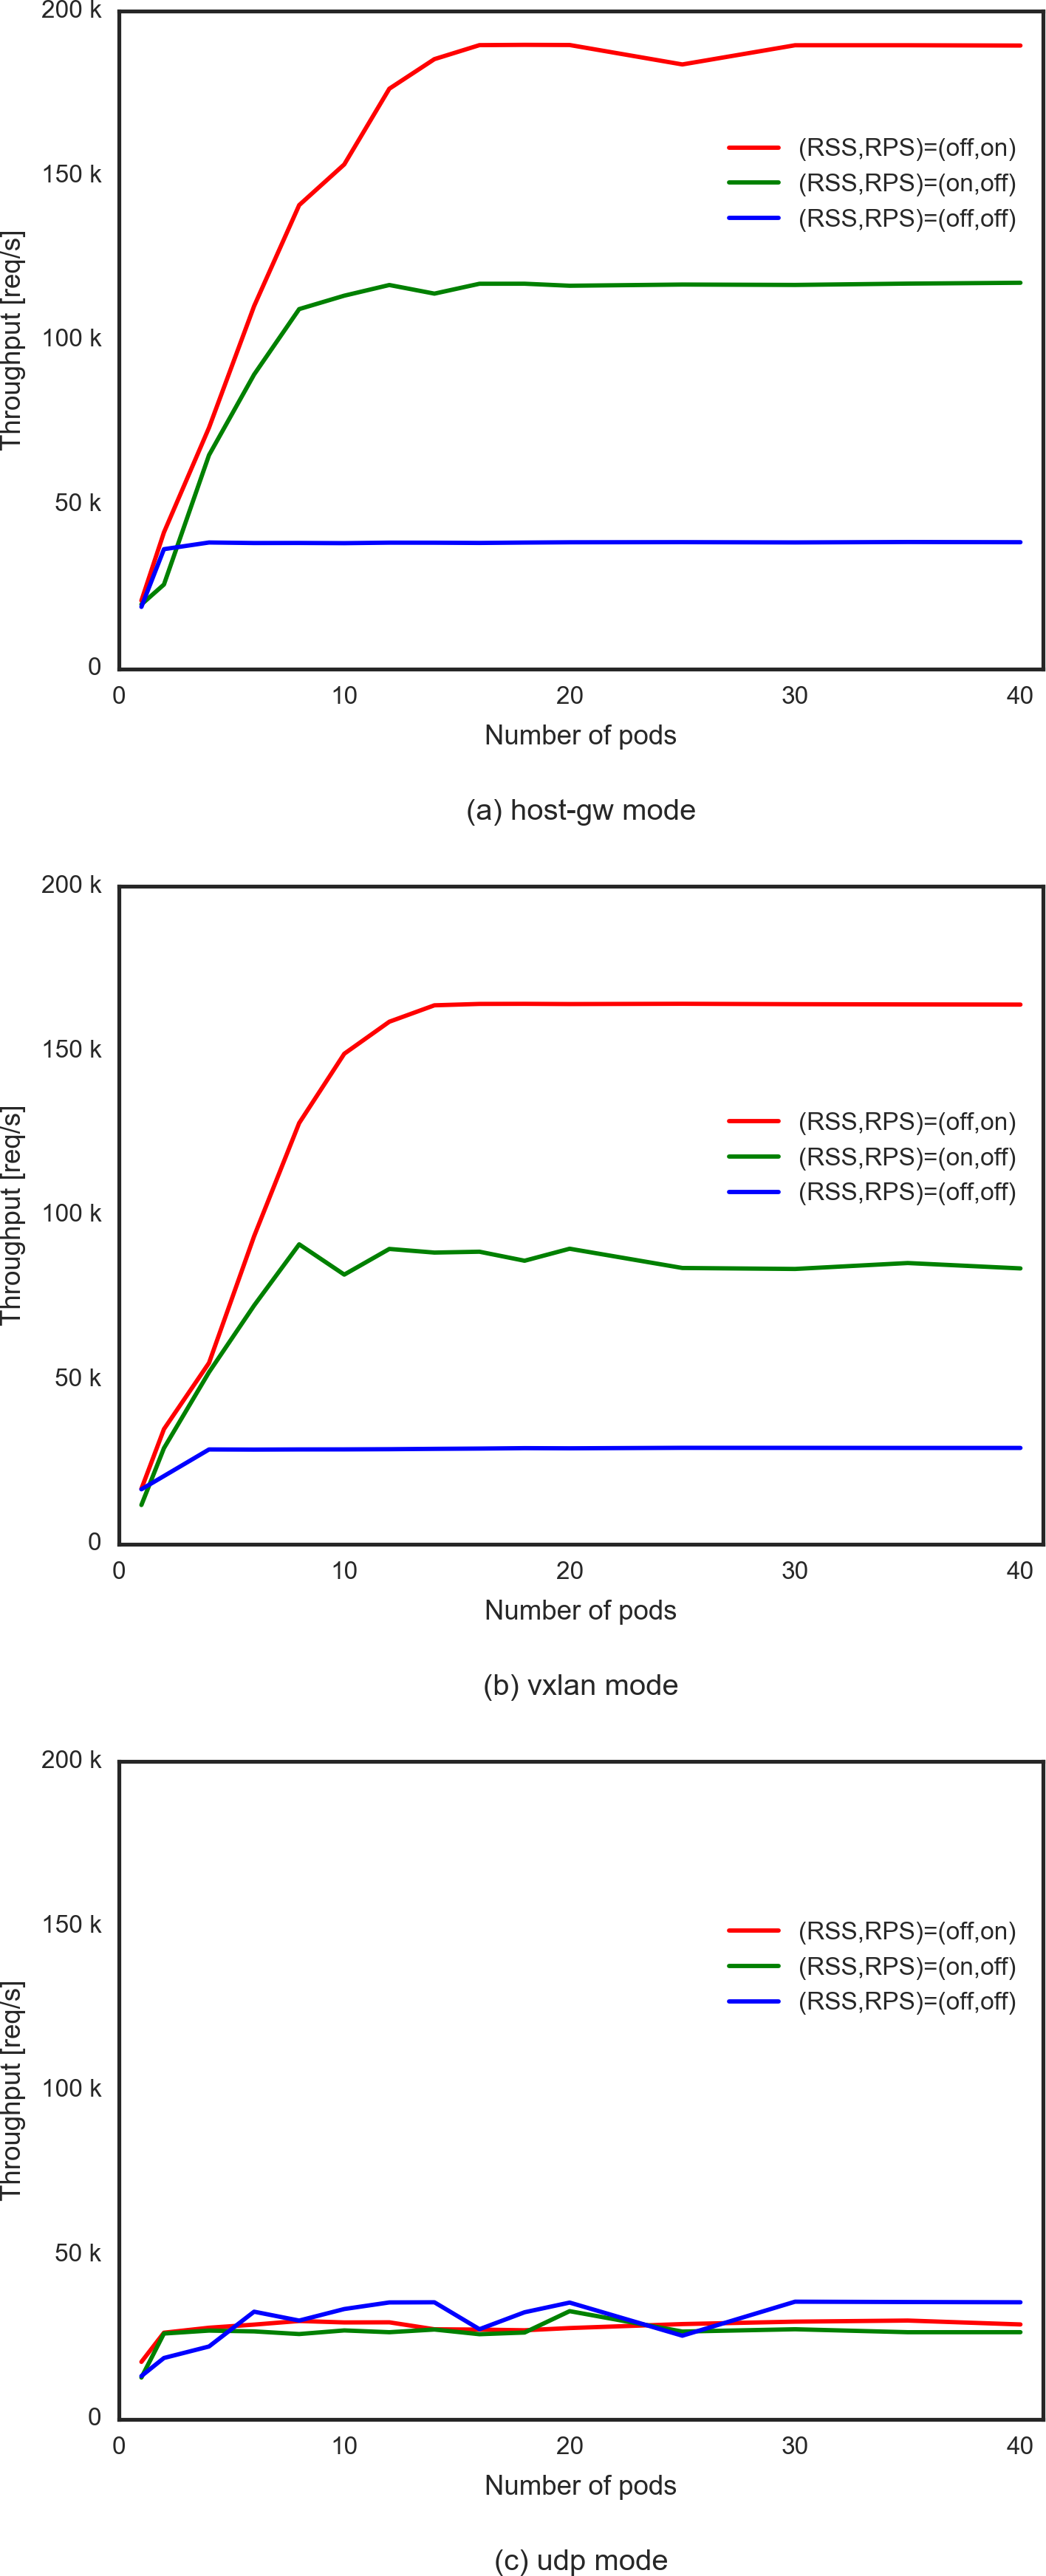
\includegraphics[width=\textwidth]{Figs/ipvs_3figs}
\caption{ipvs results}
\label{fig:ipvs3figs}
\end{figure*}

\begin{figure*}
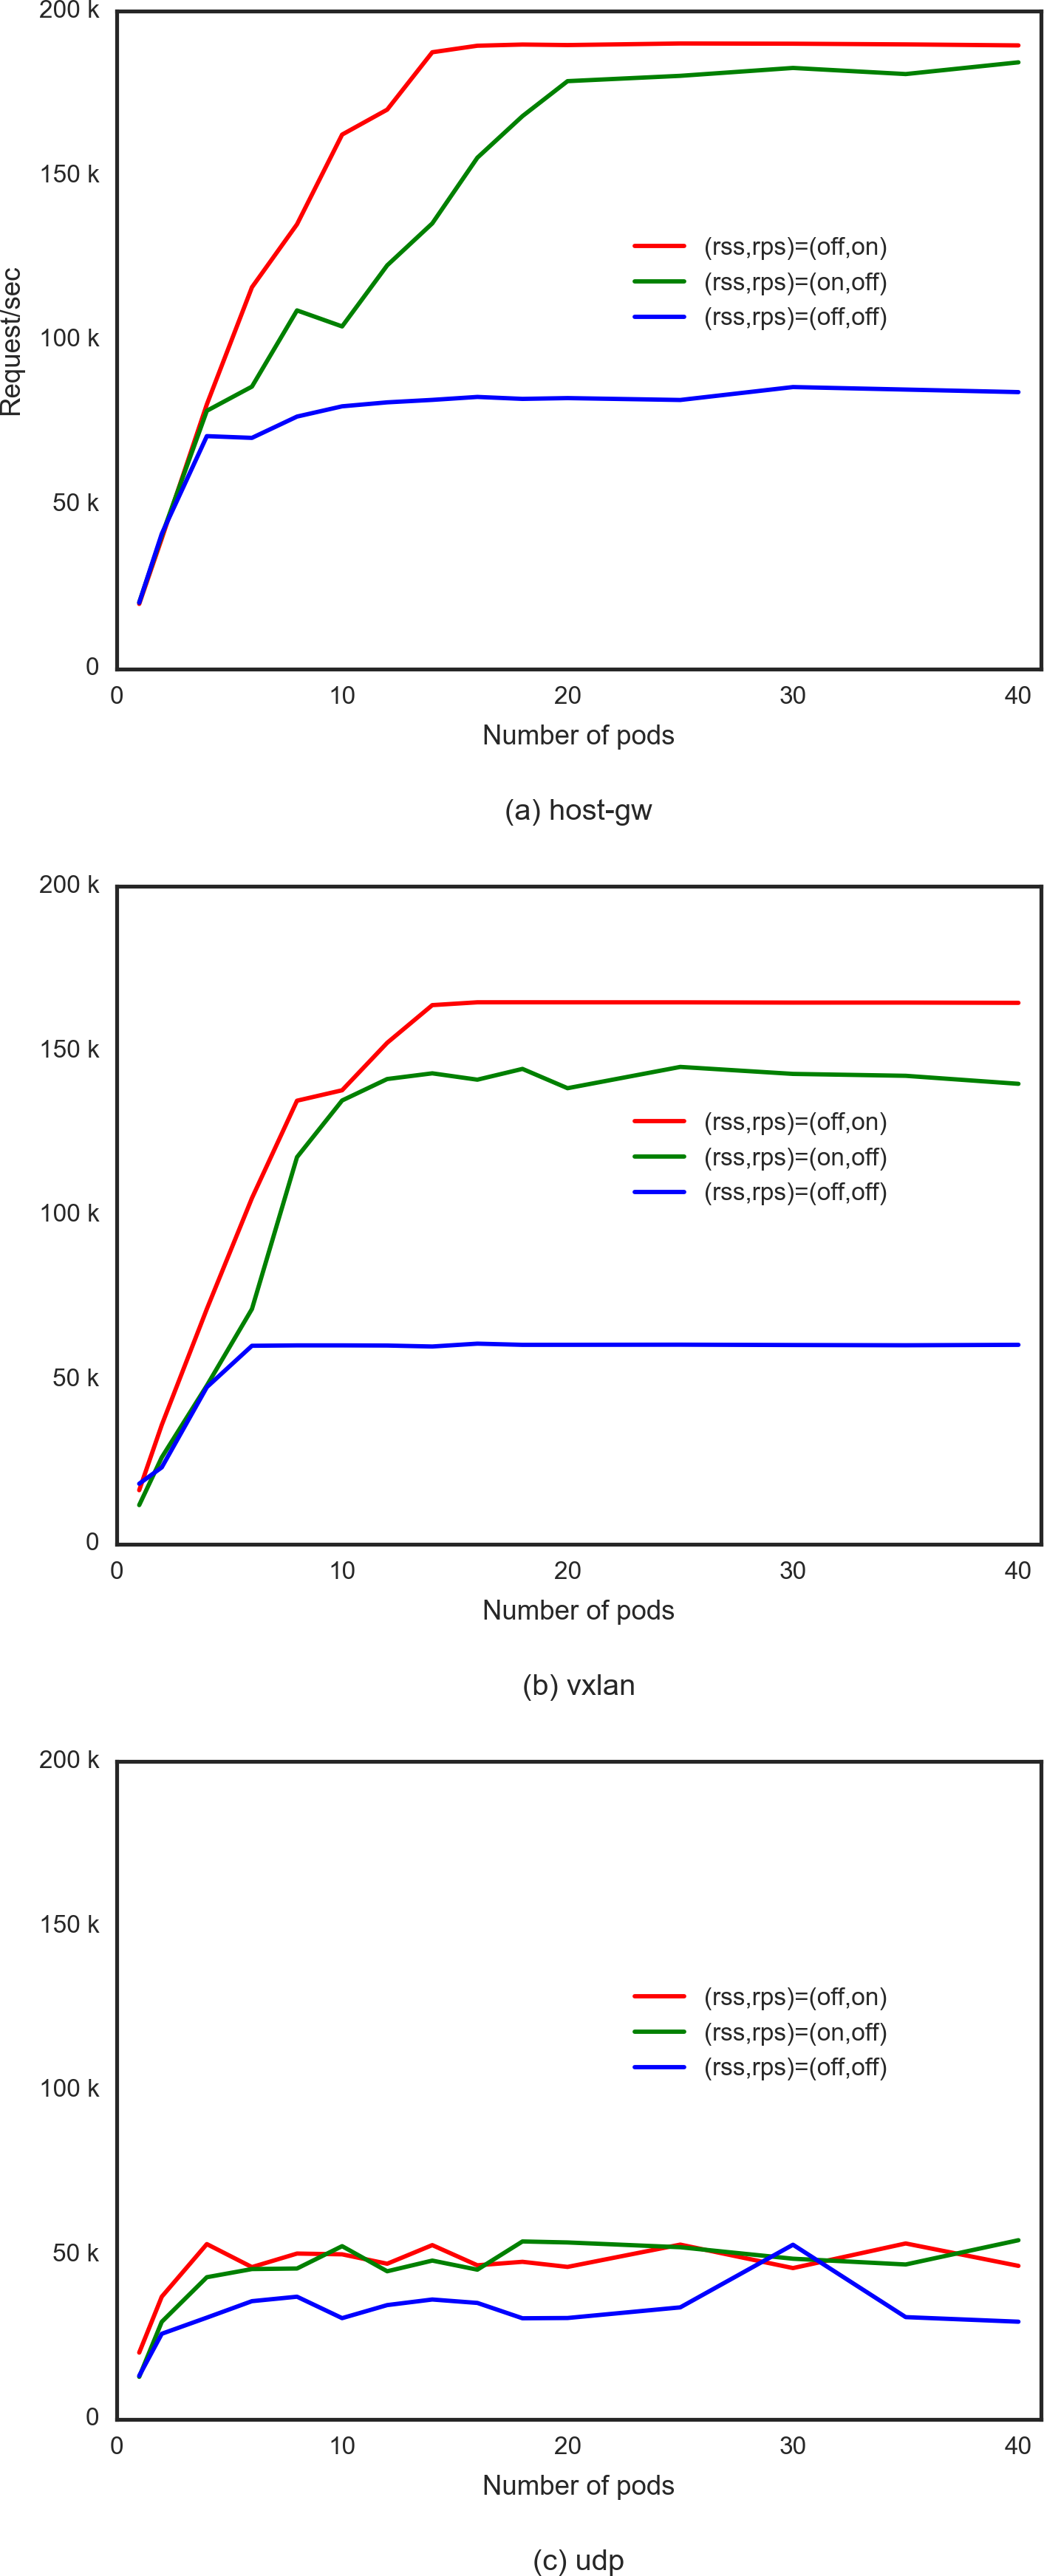
\includegraphics[width=\textwidth]{Figs/iptables_3figs}
\caption{iptables results}
\label{fig:iptabls3figs}
\end{figure*}


\begin{figure}
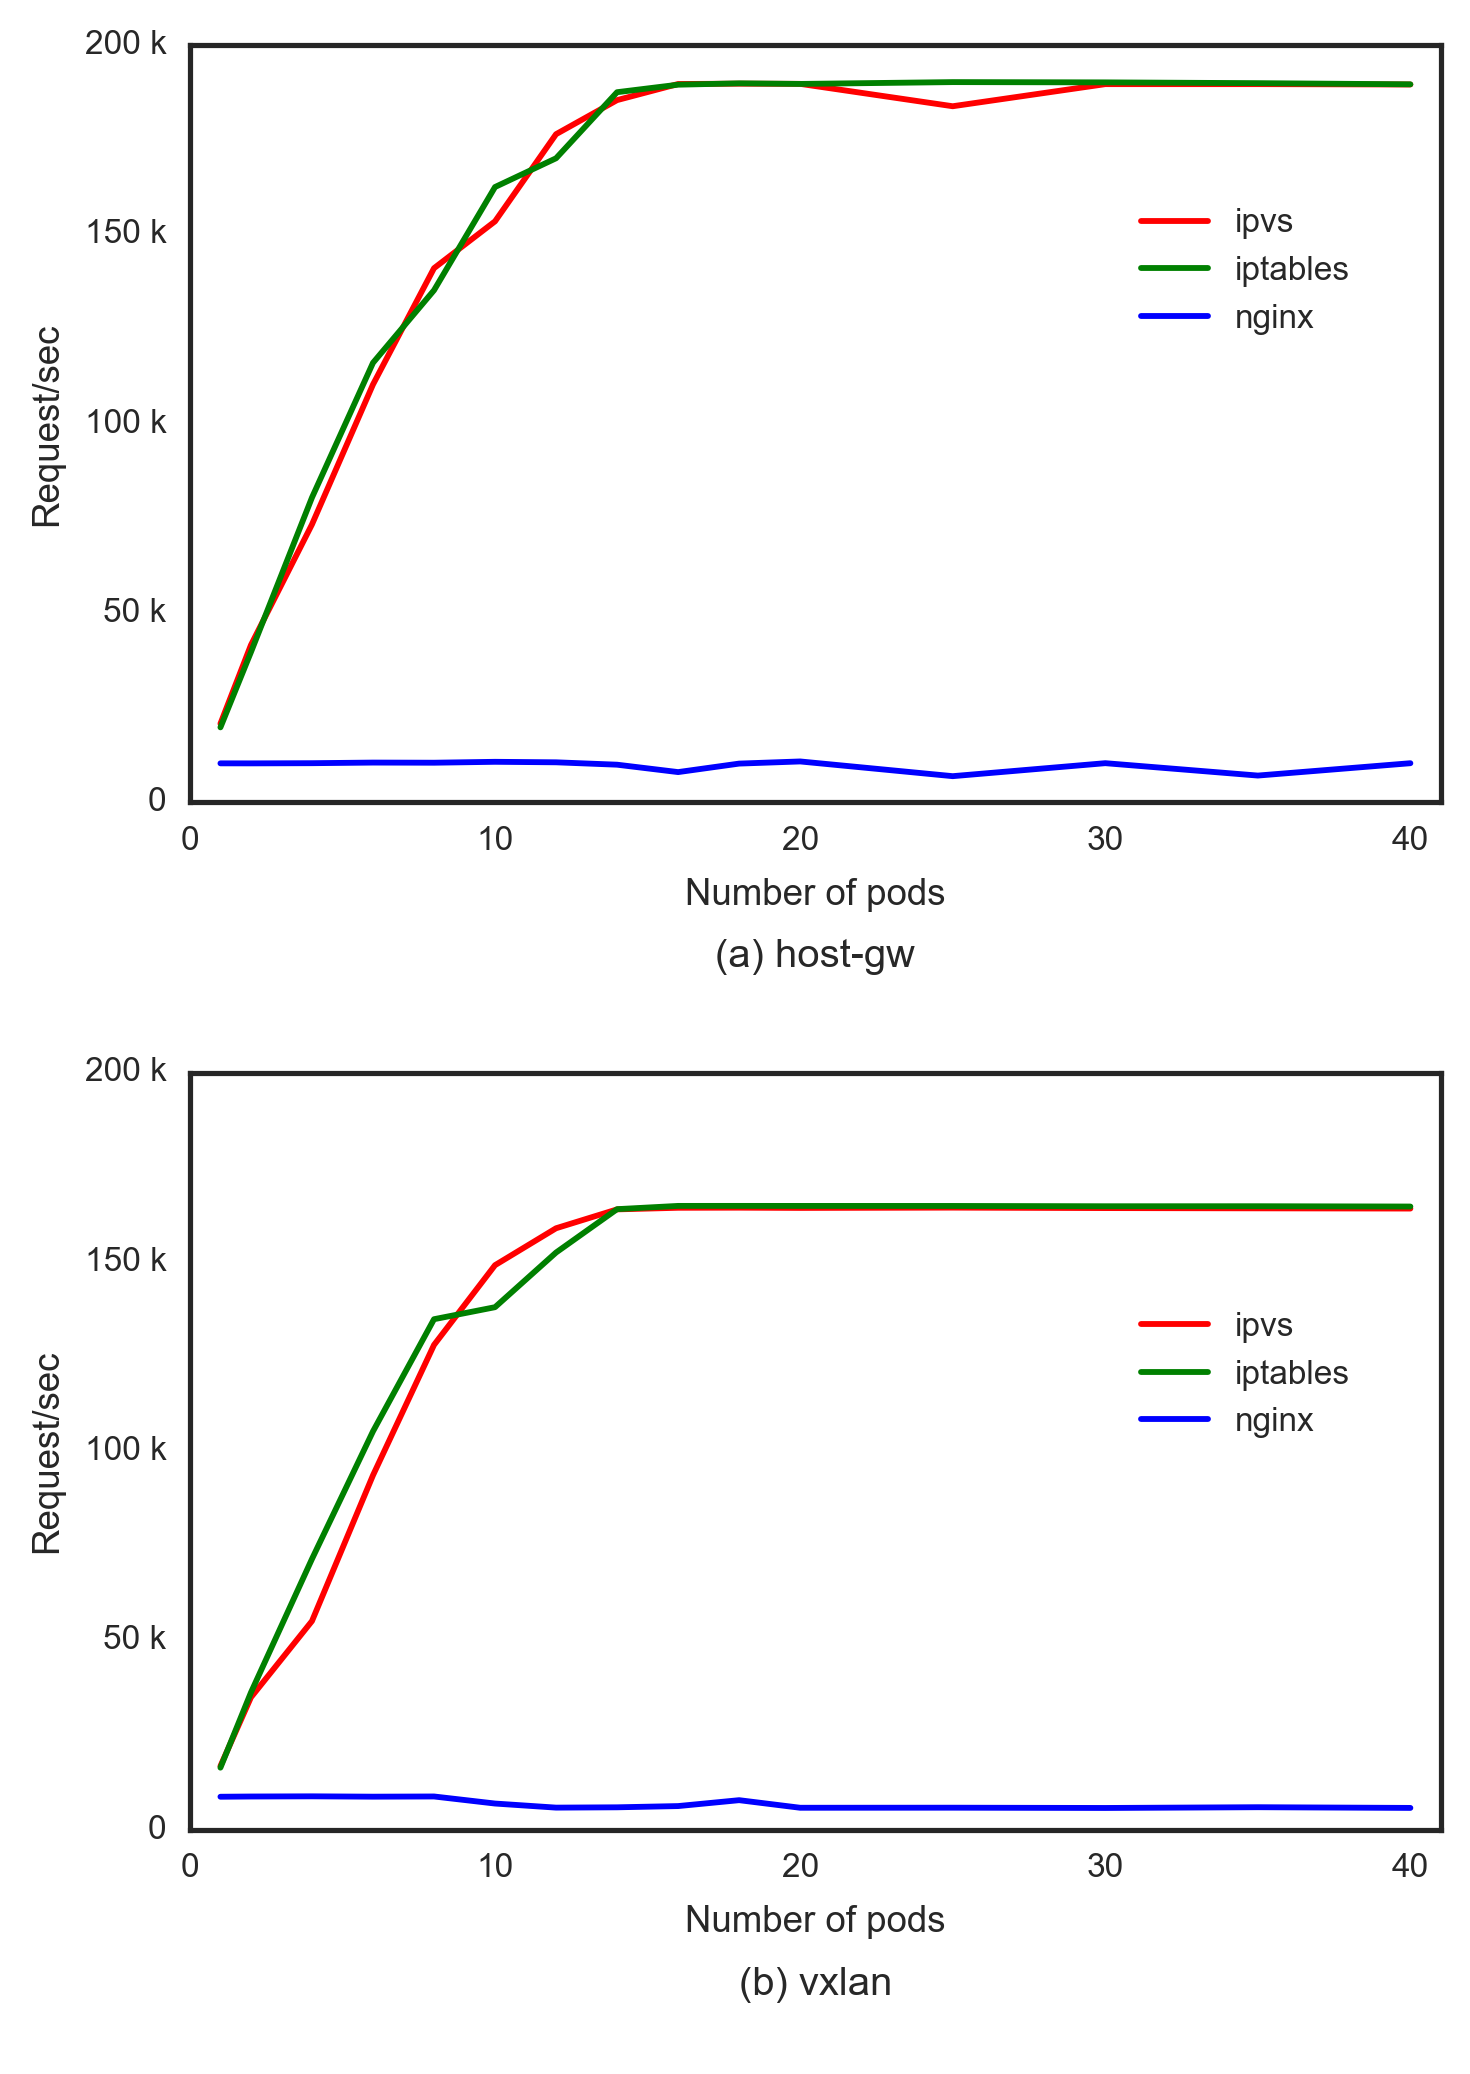
\includegraphics[width=\columnwidth]{Figs/ipvs-iptables-nginx_2figs}
\caption{ipvs and iptables comparison}
\label{fig:ipvs-iptables-nginx_2figs}
\end{figure}

Figure~\ref{fig:ipvs3figs} shows benchmark results for ipvs load balancer. 
All of them shows the performance in terms of Request/sec as a function of the number of nginx web server pods.
As for the overlay network, we measured the performance for 3 backend mode of the flannel, 
host-gw(Figure~\ref{fig:ipvs3figs}(a)), vxlan(Figure~\ref{fig:ipvs3figs}(b)) and udp(Figure~\ref{fig:ipvs3figs}(c)).

The rss and rps settings compared are the followings: 

\begin{center}
\begin{minipage}{0.8\columnwidth}
\begin{verbatim}

(rss, rps) = (off, off)
           = (on , off)
           = (off, on )

\end{verbatim}
\end{minipage}
\end{center}

Except for the udp cases, there seems to exist general tendency, 
where as the pod number increases the resulting performance increases linearly to some point, 
then eventually saturate.

Those saturated performance indicate the maximum performance of ipvs load balancer.
What limits the maximum performance depends on the flannel backend type and on the (rss, rps) settings.
From the results in Figures~\ref{fig:ipvs3figs}(a,b), if we turn off distributed packet processing,
{\it i.e.} when \enquote{(rss, rps) = (off, off)}, the performance significantly degrades. 
In this case the bottleneck of the performance is mainly due to single core packet processing.

If we compare the results for the cases when \enquote{(rss, rps) = (on, off)} and \enquote{(rss, rps) = (off, on)},
the latter is better than the former.
It is understandable, since in the case of \enquote{rps = on}, 8 physical cores are used whereas 
in the case of \enquote{rss = on} only 4 cores are used on the hardware used in our experiment.

The performance bottleneck of the case when \enquote{rss = on} is considered 
to be due to the fact that the packet processing is done on only 4 CPU cores.
What limit the performance for the case when \enquote{rps = on} is not clear yet.

If we compare the performance among the type of the flannel backend, 
the host-gw where no encapsulation is conducted has the highest performance,
followed by the vxlan where the Linux kernel encapsulate the Ethernet frame.
The udp where flanneld itself encapsulate the IP packet has the significantly lower performances.

Figure~\ref{fig:iptabls3figs} show the benchmark results for the load balancer 
functionality of the iptables DNAT. 
The performance value increases as the number of the pod increases linearly, 
then at some point comes to the saturation, as was the case with ipvs results.

If we compare the results for different packet handling settings, the highest performance is 
obtained for the case when \enquote{(rss, rps) = (off on)}, followed by the case when \enquote{(rss, rps) = (on, off)}. 
The performance result for the case when \enquote{(rss, rps) = (off, off)} resulted in the 
poorest performance as was the case for the ipvs.

As for the type of the flannel backend, the host-gw has the highest performance followed 
bye the vxlan. The udp backend totally degrade the performance.

Figure~\ref{fig:ipvs-iptables-nginx_2figs} compares the performance measurement results 
among the load balancer type, namely, ipvs, iptables DNAT and nginx 
with the condition of \enquote{(rss, rps) = (off on)}.
The proposed ipvs load balancer has almost equivalent performance as the existing iptables 
DNAT based load balancing functionality. 

The nginx based load balancer significantly under performs compared with two other methods.
For the nginx load balancer the performance never increases even though the number of the 
nginx web servers pod is increased.
This is understandable because the nginx as the web server in our experiment only 
returns it's IP address, which is nearly the lightest workload.
The performance of the nginx as a load balancer can not be much better than that of nginx as a web server 
with lightest workload.
Therefor we can expect that the nginx as a load balancer limit the performance to it's own maximum 
even though the web server pods are added to the cluster.

\section{Conclusions}\label{Conclusions}

We proposed a portable load balancer for Kubernetes cluster system, 
which aims to enable migration of a container cluster for WEB services.
In order to discuss the feasibility of such a load balancer, we built 
Kubernetes cluster system, and carried out performance measurement.
The experimental result indicated that the proposed ipvs based load balancer
had almost similar performance as the existing iptables DNAT based load balancer functionality.
We have also learned that only the vxlan and the udp backend operation modes can be used 
in the cloud environment and that the udp backend significantly under perform the vxlan backend.

Further more we also learned that the distribution of packet processing among multiple CPUs is very important
when we need to draw a maximum performance from load balancers.


%\end{document}  % This is where a 'short' article might terminate


\begin{acks}
  The authors would like to thank lots of people.

\end{acks}
